In Hops in order to communicate with the MySQL Cluster NDB we make use
of ClusterJ \cite{clusterj}, a high level API for performing
operations on NDB. In a sense it is similar to other ORM frameworks
such as Hibernate \cite{hibernate} and EclipseLink \cite{eclipselink}
which provide an object-relational mapping but more lightweight and is
designed to provide high performance methods for storing and accessing
data on a MySQL Cluster from a Java application. Every operation on
Hops and Hops-YARN, except for the events received from the NDB Event
API, goes through ClusterJ which in turn uses the C++ NDB API. The
mapping between a table-oriented view and a Java object is done
through specially decorated interfaces. The interface must also provide signatures
for the getters and setters methods.

For example in Listing \ref{lst:clusterj_intf} is the interface for
accessing database entries for the Garbage Collector service regarding
old RPCs. The interface is annotated with the table name and contains
signatures for accessing each column of the table. The methods are
also decorated with the primary key annotation and the column
name. For every table in the database there exists such an interface
and all the operations from the Hops-YARN are done on objects defined
by the annotated interfaces. \emph{Data Transfer Object}s (DTOs) are
created from a \emph{session} object which represent a connection to
the MySQL Cluster by calling the \texttt{newInstance} method. In a
typical setup an application would have multiple sessions to the
cluster. 

\lstinputlisting[float,language=Java,frame=single,caption={ClusterJ
annotated interface},label=lst:clusterj_intf]{resources/listings/clusterj_intf.java}

Upon completion of the task discussed in the previous section, we
profiled again the commit phase of a Transaction State to discover
spots where we could possibly improve. Surprisingly we discovered that
we suffered from the overhead of creating DTOs with ClusterJ. Looking
at the results of a micro-benchmark that created and persisted a
number of DTOs was astonishing. In Figure \ref{fig:impl_dto_no_cache},
the blue line represents the time that ClusterJ needed to create the
DTO instances when calling \texttt{session.newInstance}. The yellow
line is the actual time we spent just to persist them in NDB, while
the red one is the sum of those two. Constantly we are spending more
time creating the object instances than actually persist
them. Especially, when the number of instances grows beyond 6000 the
difference is massive. Creating more than 6000 DTOs is not an extreme
scenario when we are aiming to scale Hops-YARN over 10000
NodeManagers.

\begin{figure}
\centering
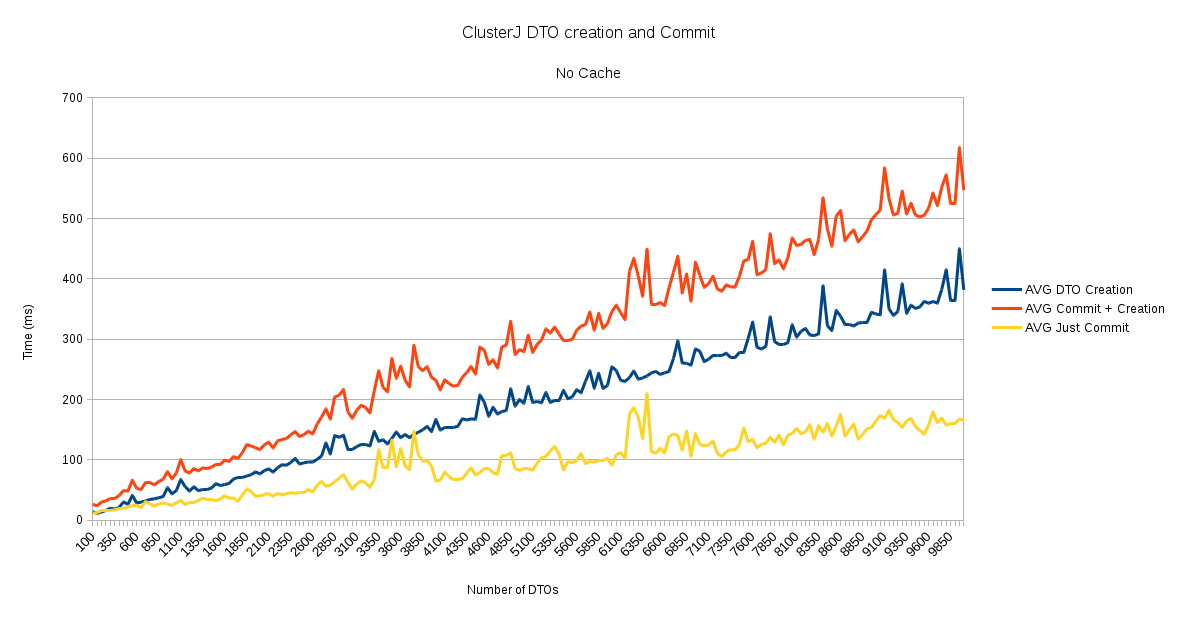
\includegraphics[scale=0.55]{resources/images/Implementation/dto_create_commit_no_cache.png}
\caption{Create and commit time for simple DTOs}
\label{fig:impl_dto_no_cache}
\end{figure}

In ClusterJ, DTOs are created from \emph{session} instances. Creation
of a new instance involves the creation of several objects such as the
handlers for the type of values the DTO will persist in NDB. Upon creation
of all the necessary handlers to check the types, it invokes the
\texttt{newInstance} reflective method of Java. Java reflection API is
a powerful tool but comes with some pitfalls including
performance \cite{java_reflection}. Reflection API loads types dynamically therefore JVM
optimizations cannot be applied making it not a good candidate for
high-performance applications. Changing the implementation of ClusterJ
is a very difficult task and was not considered as an
option. Moreover, we do not want to maintain one more project.

In Hops, ClusterJ sessions are wrapped around \emph{HopsSession}s. The
solution we designed was a DTO cache for the sessions we were
using. A session would have each own cache space that would be filled
up with instances created by the ``slow'' ClusterJ instantiation
process. When we actually needed to use a DTO, we would fetch it from
the cache which is faster since the objects would have already been
created. When the cache has been used a worker thread would fill it up
again with new instances.